\documentclass{beamer}
\mode <presentation>
{
    \usetheme{boxes}
    \usecolortheme{crane}
    \setbeamercovered{transparent}
}
\definecolor{craneorange}{RGB}{220,197, 90}


\usepackage[english]{babel}
\usepackage{times}
\usepackage{amsmath}
% math extension - one probably wants to use symbols like '[' (written as '$[$')
\usepackage{ucs}
%\usepackage[utf8]{inputenc}
\usepackage[utf8x]{inputenc}
\usepackage[normalem]{ulem}

%\setbeamercolor{background canvas}{bg=\includegraphics[width=\textwidth]{./pics/wolf.png}}

\title{Assets management with GLPI}
\author{\href{http://www.FusionInventory.org}{FusionInventory.org}}
\subject{Assets management with FusionInventory and GLPI}
\keywords{Assets management, Inventory, FusionInventory, GLPI}

\date{LinuxTag 2011}
\titlegraphic{GLPI and FusionInventory}
%subtitle{\includegraphics[width=1.2cm]{./pics/fusioninventory-logo.png}}
\institute{\includegraphics[height=3.2cm]{./pics/logos/glpi.jpg}}
\author{ Gonéri Le Bouder and Walid Nouh }
%\logo{\includegraphics[height=3.7cm]{./pics/fusinvglpi.png}}

\AtBeginSection[] % Do nothing for \section*
{
    \begin{frame}<beamer>
        \frametitle{Outline}
        \tableofcontents[currentsection]
    \end{frame}
}

%%%%%%%%%%%%%%%%%%%%%%%%%%%%%%%%%%%%%%%%%%%%%%%
%%%%%%%%%%%%%%%%%%%%%%%%%%%%%%%%%%%%%%%%%%%%%%%
\begin{document}

\frame[plain]{\titlepage}

\begin{frame}
    \frametitle{About us: Walid Nouh}
IT management consultant
    \begin{itemize}
    \item GLPI core developer
    \item FusionInventory Project co-leader
    \item ITIL expert
    \item Quad-roller fanatic
    \item Work at TECLIB', Brussels, Belgium
    \end{itemize}

\end{frame}



\begin{frame}
    \frametitle{About us: Gonéri Le Bouder}
Free software enthusiast with an awful french accent
    \begin{itemize}
    \item Debian Developer
    \item Perl Monger
    \item Former OCS Inventory developer
    \item FusionInventory Project co-leader
    \item Work at TECLIB', Paris, France
    \end{itemize}

\end{frame}


\section{Overview}


\begin{frame}
    \frametitle{Global overview}



\end{frame}

\begin{frame}
    \frametitle{Installation 1/3}

    \begin{block}{Easy step}
        \begin{itemize}
            \item Common web application
            \item Very few OS dependency
        \end{itemize}
    \end{block}

    Extract, run the wizard, your done!

\end{frame}

\begin{frame}
    \frametitle{Installation 2/3}

    \begin{block}{Easy, really? I want LDAP support! Ahah}
        \begin{itemize}
            \item Strong LDAP integration
            \item ActiveDirectory, OpenLDAP, etc support
        \end{itemize}
    \end{block}

\end{frame}

\begin{frame}
    \frametitle{Installation 3/3}

    \begin{block}{That was trivial, but I want SSO too!}
        \begin{itemize}
            \item TODO
            \item TODO
        \end{itemize}
    \end{block}

\end{frame}

\begin{frame}
    \frametitle{Architecutre}

    
\includegraphics[height=6.5cm]{pics/scale.pdf}

\end{frame}

\begin{frame}
    \frametitle{Architecutre}

    
\includegraphics[height=1.5cm]{pics/scale.pdf}
    \begin{block}{Really?}
        \begin{itemize}
            \item Existing large installation \\
            {\small up to 130K computer inventoried}
            \item 1 million computer referenced so far and counting
        \end{itemize}
    \end{block}

\end{frame}


\section{Asset Inventory}

\begin{frame}
\includegraphics[height=6.5cm]{pics/bigpicture.pdf}
\end{frame}


\begin{frame}

    \frametitle{Collect your information}


    \begin{block}{How to feed my database?}
        \begin{itemize}
            \item agent
            \item network discovery
            \item data loading
            \item financial information
            \item ...
        \end{itemize}
    \end{block}

\end{frame}

\begin{frame}

    \frametitle{Computer}

    \begin{block}{Easy step}
        \begin{itemize}
            \item Agent packaged for most of the OS
            \item Ready to use, no build, no dependency!
        \end{itemize}
    \end{block}

\end{frame}

\begin{frame}

    \frametitle{Network switch, printer, router, etc?}

    \begin{block}{FusionInventory do it remotely for you}
        \begin{itemize}
            \item Nothing to install
            \item Network scan to identify asset
            \item Use SNMP to collect information
        \end{itemize}
    \end{block}

\end{frame}

\begin{frame}

    \frametitle{Existing Inventory system}

    \begin{block}{What about my current system?}
        \begin{itemize}
            \item Financial information
            \item License
            \item Helpdesk
        \end{itemize}
    \end{block}


    \begin{block}{Various solutions}
        \begin{itemize}
            \item SOAP interface
            \item CSV import
            \item ETL
        \end{itemize}
    \end{block}

\end{frame}



\section{HelpDesk}
\section{Reporting}
\section{Questions}

\begin{frame}
    \frametitle{Questions?}

%    \bf{Questions?}
    \begin{center}

    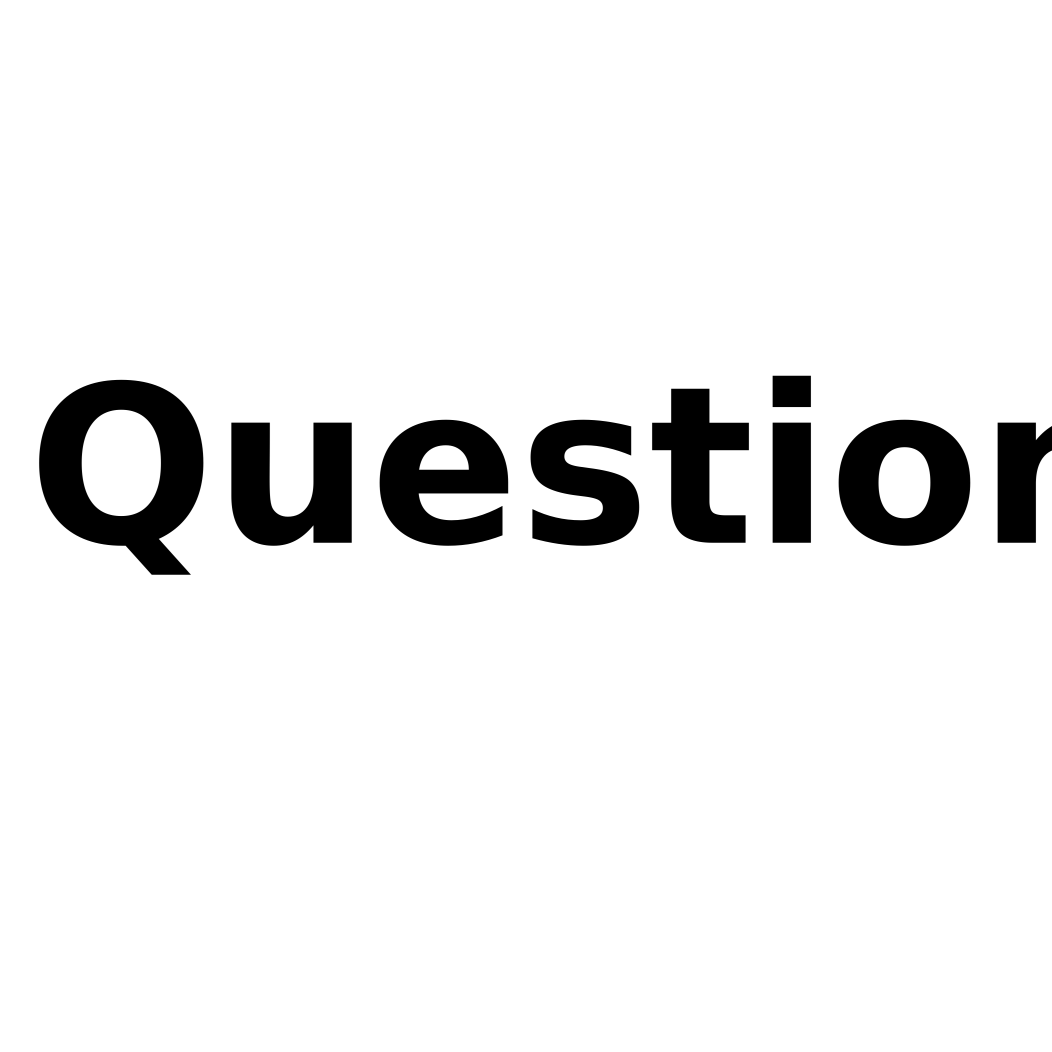
\includegraphics[height=5cm]{./pics/question.pdf}

    \end{center}
%    \includegraphics[height=7.5cm]{./pics/ask.jpg}

\end{frame}

\end{document}
